\begin{name}
	{\tenchude}
	{\tendethi}
	{ĐỀ ÔN TẬP SỐ 1}
	{\thoigian}
\end{name}
	\setcounter{ex}{0}\setcounter{bt}{0}
	\Opensolutionfile{ans}[ans/ans-2-GHK1-23-TamDuong-VinhPhuc-21]
\begin{ex}%[Đề thi HK1, Trường THPT Tam Dương, Vĩnh Phúc năm 2020-2021]%[Dự án 12EX3-Nguyễn Anh Quốc]%[2D1Y2-1]
	\immini{	Cho hàm số $y=ax^4+bx^2+c$, $(a,b,c\in \mathbb{R})$ có đồ thị như hình vẽ bên. Số điểm cực trị của hàm số là?
		\choice
		{\True $3$}
		{$2$}
		{$1$}
		{$0$}}
	{\begin{tikzpicture}[scale=1,>=stealth, font=\footnotesize, line join=round, line cap=round]
		\def\a{1} \def\b{-2} \def\c{-1} % Hệ số
		\def\xmin{-2.5} \def\xmax{2.5}
		\def\ymin{-2.5} \def\ymax{2.5} 
		%\draw[color=gray!50,dashed] (\xmin,\ymin) grid (\xmax,\ymax); 
		\draw[->] (\xmin,0)--(\xmax,0) node [below]{$x$};
		\draw[->] (0,\ymin)--(0,\ymax) node [left]{$y$};
		\node at (0,0) [below left]{$O$};
		\clip (\xmin+0.1,\ymin+0.1) rectangle (\xmax-0.5,\ymax-0.1);
		\draw[smooth,samples=300] plot(\x,{\a*(\x)^4+\b*(\x)^2+\c});
		\begin{scope}\path[white]node{MDD-108};\end{scope}
\end{tikzpicture}}
	\loigiai{
		Dựa vào đồ thị số điểm cực trị của hàm số là $3$.	
	}
\end{ex}

\begin{ex}%[Đề thi HK1, Trường THPT Tam Dương, Vĩnh Phúc năm 2020-2021]%[Dự án 12EX3-Nguyễn Anh Quốc]%[2D2Y4-2]
	Hàm số $y=2^{x^2-x}$ có đạo hàm là	
	\choice
	{$2^{x^2-x}\ln 2$}
	{\True $(2x-1)2^{x^2-x}\ln 2$}
	{$\left(x^2-x\right)2^{x^2-x-1}$}
	{$(2x-1)2^{x^2-x}$}
	\loigiai{
		Ta có $y'=\left(x^2-x\right)'2^{x^2-x}\ln 2=\left(2x-1\right)2^{x^2-x}\ln 2$.
	}
\end{ex}

\begin{ex}%[Đề thi HK1, Trường THPT Tam Dương, Vĩnh Phúc năm 2020-2021]%[Dự án 12EX3-Nguyễn Anh Quốc]%[2H1Y1-2]
	\immini{ Hình đa diện trong hình vẽ bên dưới có bao nhiêu mặt?	
		\choice
		{$6$}
		{ $12$}
		{\True $11$}
		{$10$}}
	{\begin{tikzpicture}[scale=0.4, font=\footnotesize, line join=round, line cap=round, >=stealth]
		\tkzDefPoints{0/0/a, 1/6/s, 0/1/a', 2/0.2/b, 2/1.3/b', 3/1.2/c, 3/2.2/c', -0.5/1.2/d, -0.5/2.2/d', -2.5/0.5/e, -2.5/1.5/e'}
		\tkzDrawSegments[dashed](e,d d,c e',d' d',c' d,d' s,d')
		\tkzDrawSegments(s,a' s,b' s,c' s,e' a,a' b,b' c,c' e,e' a,b b,c a,e a',e' a',b' b',c')
		\begin{scope} \path[white]node{MDD-108};\end{scope}
\end{tikzpicture}}
	\loigiai{
		Hình đa diện trên có $11$ mặt.	
	}
\end{ex}

\begin{ex}%[Đề thi HK1, Trường THPT Tam Dương, Vĩnh Phúc năm 2020-2021]%[Dự án 12EX3-Nguyễn Anh Quốc]%[2H1Y3-2]
	Khối lập phương cạnh $2a$ có thể tích là	
	\choice
	{$a^2$}
	{\True $8a^3$}
	{$6a^3$}
	{$4a^3$}
	\loigiai{
		Thể tích khối lập phương cạnh $2a$ là $V=(2a)^3=8a^3$.	
	}
\end{ex}

\begin{ex}%[Đề thi HK1, Trường THPT Tam Dương, Vĩnh Phúc năm 2020-2021]%[Dự án 12EX3-Nguyễn Anh Quốc]%[2H1Y3-2]
	Cho khối chóp có diện tích đáy $B=6a^2$ và chiều cao $h=2a$. Thể tích khối chóp đã cho bằng 	
	\choice
	{$2a^3$}
	{\True $4a^3$}
	{$6a^3$}
	{$12a^3$}
	\loigiai{
		Thể tích khối chóp là $V=\dfrac{1}{3}Bh=\dfrac{1}{3}\cdot 6a^2\cdot 2a=4a^3$.	
	}
\end{ex}

\begin{ex}%[Đề thi HK1, Trường THPT Tam Dương, Vĩnh Phúc năm 2020-2021]%[Dự án 12EX3-Nguyễn Anh Quốc]%[2D1Y1-2]
	Cho hàm số $f(x)$ có bảng biến thiên như sau
	\begin{center}
		
\begin{tikzpicture}
		\tkzTabInit[nocadre=false,lgt=1.2,espcl=2.5,deltacl=0.6]
		{$x$ /0.6,$y'$ /0.6,$y$ /2}
		{$-\infty$,$-1$,$0$,$1$,$+\infty$}
		\tkzTabLine{,+,$0$,-,$0$,+,$0$,-,}
		\tkzTabVar{-/$-\infty$, +/$2$,-/$1$,+/$2$,-/$-\infty$}
		\begin{scope} \path[white]node{MDD-108};\end{scope}
\end{tikzpicture}
	\end{center}	
	hàm số đồng biến trên khoảng nào?
	\choice
	{\True $(0;1)$}
	{$(-1;0)$}
	{$(-1;1)$}
	{$(1;+\infty)$}
	\loigiai{
		Dựa vào bảng biến thiên ta thấy hàm số đồng biến trên $(-\infty;-1)$, $(0;1)$.	
	}
\end{ex}

\begin{ex}%[Đề thi HK1, Trường THPT Tam Dương, Vĩnh Phúc năm 2020-2021]%[Dự án 12EX3-Nguyễn Anh Quốc]%[2D1Y4-1]
	Tiệm cận ngang của đồ thị hàm số $y=\dfrac{x+1}{x-1}$ là	
	\choice
	{$x=1$}
	{\True $y=1$}
	{$y=0$}
	{$y=2$}
	\loigiai{
		Tìm cận ngang của  đồ thị hàm số là $y=1$.	
	}
\end{ex}

\begin{ex}%[Đề thi HK1, Trường THPT Tam Dương, Vĩnh Phúc năm 2020-2021]%[Dự án 12EX3-Nguyễn Anh Quốc]%[2D1Y1-2]
	Cho hàm số $y=f(x)$ có bảng xét dấu đạo hàm như sau
	\begin{center}
		
\begin{tikzpicture}
		\tkzTabInit[nocadre=false,lgt=1.2,espcl=2.5,deltacl=0.6]
		{$x$ /0.6,$y'$ /0.6}
		{$-\infty$,$-2$,$0$,$2$,$+\infty$}
		\tkzTabLine{,+,$0$,-,d,-,$0$,+,}
		\begin{scope} \path[white]node{MDD-108};\end{scope}
\end{tikzpicture}
	\end{center}
	Mệnh đề nào dưới đây đúng?	
	\choice
	{Hàm số đồng biến trên khoảng $(-2;0)$}
	{\True Hàm số nghịch biến trên khoảng $(0;2)$}
	{Hàm số nghịch biến trên khoảng $(-\infty;0)$}
	{Hàm số nghịch biến trên khoảng $(-\infty;-2)$}
	\loigiai{
		Dựa vào bảng xét dấu đạo hàm ta thấy.
		\begin{itemize}
			\item  Hàm số đồng biến trong $(-\infty;-2)$, $(2;+\infty)$.
			\item Hàm số nghịch biến trong $(-2;0)$, $(0;2)$.
		\end{itemize}
	}
\end{ex}

\begin{ex}%[Đề thi HK1, Trường THPT Tam Dương, Vĩnh Phúc năm 2020-2021]%[Dự án 12EX3-Nguyễn Anh Quốc]%[2D1Y5-3]
	Cho hàm số $f(x)$ có bảng biến thiên như sau
	\begin{center}
		
\begin{tikzpicture}
		\tkzTabInit[nocadre=false,lgt=1.2,espcl=2.5,deltacl=0.6]
		{$x$ /0.6,$f'(x)$ /0.6,$f(x)$ /2}
		{$-\infty$,$-2$,$0$,$2$,$+\infty$}
		\tkzTabLine{,-,$0$,+,$0$,-,$0$,+,}
		\tkzTabVar{+/$+\infty$, -/$-1$,+/$2$,-/$-1$,+/$+\infty$}
		\begin{scope} \path[white]node{MDD-108};\end{scope}
\end{tikzpicture}
	\end{center}	
	Số nghiệm của phương trình $f(x)-1=0$ là
	\choice
	{$2$}
	{$0$}
	{\True $4$}
	{$3$}
	\loigiai{
		Ta thấy $f(x)-1=0\Leftrightarrow f(x)=1$. Đây là phương trình hoành độ giao điểm của đồ thị hàm số $y=f(x)$ và $y=1$. Dựa vào bảng biến thiên ta thấy phương trình có $4$ nghiệm phân biệt.	
	}
\end{ex}

\begin{ex}%[Đề thi HK1, Trường THPT Tam Dương, Vĩnh Phúc năm 2020-2021]%[Dự án 12EX3-Nguyễn Anh Quốc]%[2H1Y2-2]
	Số cạnh của một hình bát diện đều là	
	\choice
	{$10$}
	{$8$}
	{$6$}
	{\True $12$}
	\loigiai{
		Số cạnh của một hình bát diện đều là $12$.	
	}
\end{ex}

\begin{ex}%[Đề thi HK1, Trường THPT Tam Dương, Vĩnh Phúc năm 2020-2021]%[Dự án 12EX3-Nguyễn Anh Quốc]%[2D1Y1-1]
	Cho hàm số $f(x)=\dfrac{2x+3}{x-1}$, hàm số nghịch biến trên khoảng nào?
	\choice
	{$(-\infty;+\infty)$}
	{$(-\infty;1)$}
	{$(1;+\infty)$}
	{\True $(-\infty;1)$ và $(1;+\infty)$}
	\loigiai{
		Tập xác định của hàm số là $\mathscr{D}=\mathbb{R}\setminus\{1\}.$\\
		Ta có $y'=\dfrac{-5}{(x-1)}<0,\forall x\in \mathscr{D}$.\\
		Vậy hàm số nghịch biến trên từng khoảng $(-\infty;1)$ và $(1;+\infty)$.	
	}
\end{ex}

\begin{ex}%[Đề thi HK1, Trường THPT Tam Dương, Vĩnh Phúc năm 2020-2021]%[Dự án 12EX3-Nguyễn Anh Quốc]%[2D1Y2-2]
	Cho hàm số $y=f(x)$ có bảng biến thiên như sau
	\begin{center}
		
\begin{tikzpicture}
		\tkzTabInit[nocadre=false,lgt=1.2,espcl=2.5,deltacl=0.6]
		{$x$ /0.6, $y'$ /0.6, $y$ /2.5}
		{$-\infty$,$-1$,$2$,$+\infty$}
		\tkzTabLine{,+,$0$,-,$0$,+,}
		\tkzTabVar{-/$2$,+/$4$,-/$-5$,+/$2$}
		\begin{scope} \path[white]node{MDD-108};\end{scope}
\end{tikzpicture}
	\end{center}	
	Mệnh đề nào dưới đây đúng?
	\choice
	{Hàm số có bốn điểm cực trị}
	{\True Hàm số đạt cực tiểu tại $x=2$}
	{Hàm số không có điểm cực đại}
	{Hàm số đạt cực tiểu tại $x=-5$}
	\loigiai{
		Dựa vào bảng biến thiên ta thấy hàm số đạt cực tiểu tại $x=2$.	
	}
\end{ex}

\begin{ex}%[Đề thi HK1, Trường THPT Tam Dương, Vĩnh Phúc năm 2020-2021]%[Dự án 12EX3-Nguyễn Anh Quốc]%[2D2Y1-2]
	Rút gọn biểu thức $a^{\frac{3}{2}}	\cdot a^3$ ta được
	\choice
	{$a^{\frac{1}{2}}$}
	{\True $a^{\frac{9}{2}}$}
	{$a^{\frac{9}{4}}$}
	{$a^{4}$}
	\loigiai{
		Ta có $a^{\frac{3}{2}}\cdot	a^3=a^{\frac{3}{2}+3}=a^{\frac{9}{2}}.$
	}
\end{ex}

\begin{ex}%[Đề thi HK1, Trường THPT Tam Dương, Vĩnh Phúc năm 2020-2021]%[Dự án 12EX3-Nguyễn Anh Quốc]%[2D1Y5-1]
	\immini{Đồ thị của hàm số nào dưới đây có dạng như đường cong trong hình vẽ bên?	
		\choice
		{$y=x^3-3x+1$}
		{\True $y=-x^3+3x+1$}
		{$y=x^4-2x^2+1$}
		{$y=-x^4+2x^2+1$}}{
		\begin{tikzpicture}[scale=0.8,>=stealth, font=\footnotesize, line join=round, line cap=round]
		\def\a{-1} \def\b{0} \def\c{3} \def\d{1} % Hệ số
		\def\xmin{-3} \def\xmax{3}
		\def\ymin{-2} \def\ymax{4} 
		% \draw[color=gray!50,dashed] (\xmin,\ymin) grid (\xmax,\ymax); 
		\draw[->] (\xmin,0)--(\xmax,0) node [below]{$x$};
		\draw[->] (0,\ymin)--(0,\ymax) node [left]{$y$};
		\node at (0,0) [below right]{$O$};
		\clip (\xmin+0.1,\ymin+0.1) rectangle (\xmax-0.5,\ymax-0.1);
		\draw[smooth,samples=300] plot(\x,{\a*(\x)^3+\b*(\x)^2+\c*(\x)+\d});
		\begin{scope} \path[white]node{MDD-108};\end{scope}
\end{tikzpicture}
	}
	\loigiai{
		Đồ thị đã cho làm hàm số bậc ba nên ta loại $y=x^4-2x^2+1$, $y=-x^4+2x^2+1$. Mặt khác $\displaystyle\lim\limits_{x\to +\infty}y=-\infty$ nên $a<0$, do đó ta loại $y=x^3-3x+1$.
	}
\end{ex}

\begin{ex}%[Thi thử lần 2, Sở GD và ĐT - Vĩnh Phúc, PTTH Tam dương, 2020-2021]%[nguyễn hoàng thanh, 12EX3]%[2H1Y3-2]
	Cho khối chóp có đáy là hình vuông cạnh $ a $ và chiều cao bằng $2a $. Thể tích của khối chóp đã cho bằng?
	\choice
	{$ 4a^3 $}
	{$ \dfrac{4}{3}a^3 $}
	{ $2a^3 $}
	{\True$ \dfrac{2}{3}a^3 $}
	\loigiai{
		Thể tích khối chóp được tính theo công thức $ V=\dfrac{1}{3}S\cdot h $.\\
		Trong đó $ S=a^2 $, $ h=2a $, suy ra $ V=\dfrac{2}{3}a^3 $.
	}
\end{ex}

\begin{ex}%[Thi thử lần 2, Sở GD và ĐT - Vĩnh Phúc, PTTH Tam dương, 2020-2021]%[nguyễn hoàng thanh, 12EX3]%[2D1Y2-2]
	\immini{Cho hàm số $ y=f(x) $ có bảng biến thiên như hình vẽ bên. Giá trị cực tiểu của hàm số đã cho bằng?
	}{
		
\begin{tikzpicture}[>=stealth,line join=round,line cap=round,font=\footnotesize,scale=0.8,smooth]
		\tkzTabInit[nocadre=false,lgt=1,espcl=2,deltacl=0.5]{$x$/.7 ,$y'$/.7,$y$/1.7}
		{$-\infty$ , $0$ , $3$ , $+\infty$}
		\tkzTabLine{ , + , $0$ , - , $0$ , + , }
		\tkzTabVar{-/$-\infty$ , +/$2$ , -/$-4$ , +/$+\infty$}
		\begin{scope} \path[white]node{MDD-108};\end{scope}
\end{tikzpicture}
	}
	\choice
	{ $2$}
	{$ 3 $}
	{$0 $}
	{\True$-4$}
	\loigiai{
		Quan sát bảng biến thiên, ta thấy giá trị cực tiểu của hàm số là $ y(3)=-4 $.
	}
\end{ex}

\begin{ex}%[Thi thử lần 2, Sở GD và ĐT - Vĩnh Phúc, PTTH Tam dương, 2020-2021]%[nguyễn hoàng thanh, 12EX3]%[2D1Y1-2]
	\immini{Cho hàm số $ y=f(x) $ có đồ thị như hình vẽ. Hàm số đã cho nghịch biến trên khoảng nào dưới đây?	
	}{
		% Đồ thị hàm y=ax^3+bx^2+cx+d. Nếu hệ số lớn cần điều chỉnh hệ trục, vùng lưới, domain và lệnh \clip
		\begin{tikzpicture}[>=stealth,line join=round,line cap=round,font=\footnotesize,scale=0.8,smooth]
		\draw[->] (-2,0)--(0,0) node[below right]{O}-- (3,0)node[below]{\scriptsize $x$};
		\draw[->] (0,-1)--(0,1) node[below right]{$ 1 $}-- (0,4) node[left] {\scriptsize $y$};
		\draw[] plot[smooth,tension=.6] coordinates{(-.6,3)(0,1)(1,2)(1.7,-.5)};
		\draw[dashed] (1,0)node[below]{$ 1 $}--(1,2)--(0,2)node[above right]{$2$};
		\begin{scope} \path[white]node{MDD-108};\end{scope}
\end{tikzpicture}
	}
	\choice
	{$ (0;+\infty) $}
	{$ (-\infty;1) $}
	{\True$ (2;+\infty) $}
	{ $ (0;1) $}
	\loigiai{
		Quan sát đồ thị hàm số, ta thấy hàm số nghịch biến trên khoảng $ (-\infty;0) $, $ (2;+\infty) $. 
	}
\end{ex}

\begin{ex}%[Thi thử lần 2, Sở GD và ĐT - Vĩnh Phúc, PTTH Tam dương, 2020-2021]%[nguyễn hoàng thanh, 12EX3]%[2H2Y2-1]
	Thể tích của khối cầu bán kính $ R $ bằng
	\choice
	{$\dfrac{3}{4}\pi R^3$}
	{\True$\dfrac{4}{3}\pi R^3$}
	{$4\pi R^3$}
	{$2\pi R^3$}
	\loigiai{
		Thể tích khối cầu bán kính $ R $ là $ V=\dfrac{4}{3}\pi R^3 $.
	}
\end{ex}

\begin{ex}%[Thi thử L2, Chuyển đề THPT Tam Dương - Vĩnh Phúc, 2021]%[Quan Văn Ón,12EX-3-2021]%[2H2Y1-2]
	Diện tích xung quanh của hình trụ tròn xoay có bán kính đáy $r$ và độ dài đường sinh $l$ bằng
	\choice
	{$4\pi rl$}
	{\True $2\pi rl$}
	{$\dfrac{4}{3}\pi rl$}
	{$\pi rl$}
	\loigiai{
		\immini{
			Diện tích xung quanh của hình trụ tròn xoay có bán kính đáy $r$ và độ dài đường sinh $l$ là $S_{xq} = 2\pi rl$.
		}{
			\begin{tikzpicture}[scale=0.6, font=\footnotesize, line join=round, line cap=round, >=stealth]
			\draw[dashed] (3,0) arc (0:180:3 cm and 1cm);
			\draw (3,0) arc (0:-180:3 cm and 1cm);
			\draw (3,4) arc (0:360:3 cm and 1cm);
			\tkzDefPoints{0/0/O,0/4/O',-3/0/A,3/0/B,3/4/C,-3/4/D}
			\tkzDrawPoints[fill=black](O,O')
			\tkzDrawSegments[dashed](O,O')
			\tkzDrawSegments(A,D)
			%\tkzLabelPoints(A,B,C,D)
			\tkzLabelPoints[below](O)
			\tkzLabelPoints[above](O')
			\draw (B) to node[right]{$\ell$} (C);
			\draw[dashed] (O) to node[sloped,above]{$r$} (B);
			\begin{scope} \path[white]node{MDD-108};\end{scope}
\end{tikzpicture}
		}
	}
\end{ex}

\begin{ex}%[Thi thử L2, Chuyển đề THPT Tam Dương - Vĩnh Phúc, 2021]%[Quan Văn Ón,12EX-3-2021]%[2D1Y5-1]
	Hàm số $y = ax^4 + bx^2 + c$ có đồ thị như hình vẽ bên. Mệnh đề nào sau đây là đúng?
	\begin{center}
		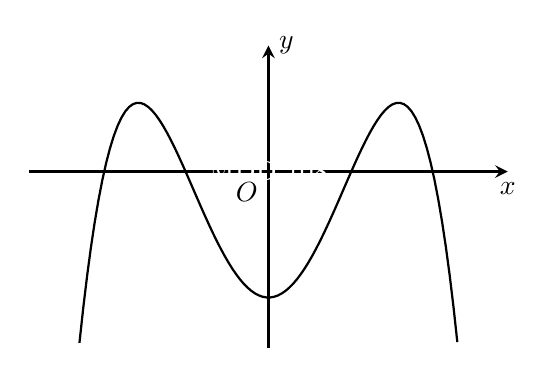
\begin{tikzpicture}[scale = 0.8,>=stealth]
		\draw[->,line width = 1pt] (-3.8,0)--(0,0) node[below left]{$O$}--(3.8,0) node[below]{$x$};
		\draw[->,line width = 1pt] (0,-2.8)--(0,2) node[right]{$y$};
		\draw [thick, domain=-3:3, samples=100] %
		plot (\x, {-0.17*(\x)^4+1.45*(\x)^2-2});
		\begin{scope} \path[white]node{MDD-108};\end{scope}
\end{tikzpicture}
	\end{center}
	\choice
	{$a < 0$, $b > 0$, $c > 0$}
	{$a < 0$, $b < 0$, $c > 0$}
	{\True $a < 0$, $b > 0$, $c < 0$}
	{$a < 0$, $b < 0$, $c < 0$}
	\loigiai{
		Vì đồ thị là của hàm trùng phương và theo hình dáng đồ thị thì $a < 0$. Đồ thị có $3$ cực trị nên $a$, $b$ trái dấu, suy ra $b > 0$. Hơn nữa, tại $x = 0$ thì $y < 0 \Rightarrow c < 0$.
	}
\end{ex}

\begin{ex}%[Đề thi HK1, Trường THPT Tam Dương, Vĩnh Phúc năm 2020-2021]%[Dự án 12EX3-Nguyễn Anh Quốc]%[2D2B4-1]
	Tìm tập xác định $\mathscr{D}$ của hàm số $y=\log_3\left(x^2-4x+3\right)$.	
	\choice
	{$\mathscr{D}=(1;3)$}
	{\True $\mathscr{D}=(-\infty;1)\cup (3;+\infty)$}
	{$\mathscr{D}=(-\infty;2-\sqrt{2})\cup (2+\sqrt{2};+\infty)$}
	{$\mathscr{D}=(2-\sqrt{2};1)\cup (3;2+\sqrt{2})$}
	\loigiai{
		Hàm số xác định khi $x^2-4x+3>0\Leftrightarrow \hoac{&x<1\\&x>3.}$\\
		Vậy tập xác định của hàm số là $\mathscr{D}=(-\infty;1)\cup (3;+\infty)$.	
	}
\end{ex}

\begin{ex}%[Đề thi HK1, Trường THPT Tam Dương, Vĩnh Phúc năm 2020-2021]%[Dự án 12EX3-Nguyễn Anh Quốc]%[2D1B4-2]
	Giá trị của $m$ để tiệm cận đứng của đồ thị hàm số $y=\dfrac{2x+1}{x+m}$ đi qua điểm $M(2;3)$ là	
	\choice
	{$-2$}
	{\True $2$}
	{$3$}
	{$0$}
	\loigiai{
		Tiệm cận đứng của đồ thị hàm số là $x=-m$, đi qua điểm $M(2;3)$ nên $2=-m\Rightarrow m=2$.	
	}
\end{ex}

\begin{ex}%[Đề thi HK1, Trường THPT Tam Dương, Vĩnh Phúc năm 2020-2021]%[Dự án 12EX3-Nguyễn Anh Quốc]%[2D1B4-3]
	\immini{ Xác định $a$, $b$ để hàm số $y=\dfrac{ax-1}{x+b}$ có đồ thị như hình vẽ bên. Mệnh đề nào sau đây đúng?	
		\choice
		{$a=1$, $b=-1$}
		{$a=-1$, $b=1$}
		{\True $a=1$, $b=1$}
		{$a=-1$, $b=-1$}}
	{\begin{tikzpicture}[scale=0.8,>=stealth, font=\footnotesize, line join=round, line cap=round]
		\def\a{1} \def\b{-1} \def\c{1} \def\d{1} % Hệ số
		\def\xmin{-4} \def\xmax{4}
		\def\ymin{-3} \def\ymax{4}
		%	\draw[color=gray!50,dashed] (\xmin,\ymin) grid (\xmax,\ymax);
		\draw[->] (\xmin,0)--(\xmax,0) node [below]{$x$};
		\draw[->] (0,\ymin)--(0,\ymax) node [left]{$y$};
		\node at (0,0) [below left]{$O$};
		\clip (\xmin+0.1,\ymin+0.1) rectangle (\xmax-0.1,\ymax-0.1);
		\draw[smooth,samples=300,domain=\xmin:(-\d/\c-0.1)] plot(\x,{(\a*(\x)+\b)/(\c*(\x)+\d)});
		\draw[smooth,samples=300,domain=(-\d/\c+0.1:\xmax)] plot(\x,{(\a*(\x)+\b)/(\c*(\x)+\d)});
		\draw[dashed] (-\d/\c,\ymin)--(-\d/\c,\ymax);
		\draw[dashed] (\xmin,\a/\c)--(\xmax,\a/\c);
		\draw (-1,0)node[below left]{$-1$}circle(1pt) (0,1)node[above right]{$1$}circle(1pt);
		\begin{scope} \path[white]node{MDD-108};\end{scope}
\end{tikzpicture}}
	\loigiai{
		Dựa vào đồ thị đường tiệm cận đứng là $x=-1$ và tiệm cận ngang là $y=1$ nên ta suy ra $a=1$, $b=1$.	
	}
\end{ex}

\begin{ex}%[Đề thi HK1, Trường THPT Tam Dương, Vĩnh Phúc năm 2020-2021]%[Dự án 12EX3-Nguyễn Anh Quốc]%[2H1B3-2]
	Một khối lập phương có độ dài đường chéo là $a\sqrt{6}$. Thể tích khối lập phương đó là
	\choice
	{\True $V=2\sqrt{2}a^3$}
	{$V=3\sqrt{3}a^3$}
	{$V=6\sqrt{6}a^3$}
	{$V=64a^3$}
	\loigiai{
		\immini{Giả sử khối lập phương đã cho là $ABCD.A'B'C'D'$, theo đề bài ta có $AC'=a\sqrt{6}$, mà $AC'=\sqrt{3}AB\Rightarrow \sqrt{3}AB=a\sqrt{6}\Rightarrow AB=a\sqrt{2}$. Thể tích khối lập phương là $V=AB^3=\left(a\sqrt{2}\right)^3=2\sqrt{2}a^3$.}
		{\begin{tikzpicture}[scale=0.8,>=stealth, font=\footnotesize, line join=round, line cap=round]
			\tkzDefPoints{0/0/A,-1.3/-1.1/B,2/-1.1/C}
			\coordinate (D) at ($(A)+(C)-(B)$);
			\coordinate (A') at ($(A)+(0,2.5)$);
			\tkzDefPointsBy[translation=from A to A'](B,C,D){B'}{C'}{D'}
			\tkzDrawPolygon(A',B',B,C,D,D')
			\tkzDrawSegments(B',C' C',D' C,C')
			\tkzDrawSegments[dashed](A,B A,D A,A')
			\tkzDrawPoints[fill=black,size=4](A,B,D,C,A',B',C',D')
			\tkzLabelPoints[above](A',D')
			\tkzLabelPoints[below](A,B,C)
			\tkzLabelPoints[left](B')
			\tkzLabelPoints[right](C',D)
			\begin{scope} \path[white]node{MDD-108};\end{scope}
\end{tikzpicture}}
	}
\end{ex}

\begin{ex}%[Đề thi HK1, Trường THPT Tam Dương, Vĩnh Phúc năm 2020-2021]%[Dự án 12EX3-Nguyễn Anh Quốc]%[2D1B3-1]
	Giá trị lớn nhất của hàm số $y=\dfrac{x+4}{x-2}$ trên đoạn $[3;5]$ bằng	
	\choice
	{$3$}
	{$-2$}
	{$5$}
	{\True $7$}
	\loigiai{
		Ta có $y'=\dfrac{-6}{(x-2)^2}<0,\forall x\in [3;5]$, suy ra hàm số nghịch biến trên $[3;5]$.\\ Do đó $\displaystyle\max\limits_{[3;5]}y=y(3)=7$.	
	}
\end{ex}

\begin{ex}%[Thi thử lần 2, Sở GD và ĐT - Vĩnh Phúc, PTTH Tam dương, 2020-2021]%[nguyễn hoàng thanh, 12EX3]%[2D1B3-1]
	Giá trị lớn nhất của hàm số $f(x)=x^4-4x^2+5 $ trên đoạn $ [-2;3] $ bằng
	\choice
	{ $ 5 $}
	{\True$ 50 $}
	{$ 1 $}
	{$122 $}
	\loigiai{
		Tập xác định $ \mathscr{D}=\mathbb{R} $.\\
		Đạo hàm $ f'(x)=4x^3-8x $.
		Cho $ f'(x)=0\Leftrightarrow 4x^3-8x=0\Leftrightarrow \hoac{&x=0\\&x=\sqrt{2}\\&x=-\sqrt{2}.}$\\
		Ta có $ \hoac{&f(-2)=5\\&f(0)=5\\&f(-\sqrt{2})=1\\&f(\sqrt{2})=1\\&f(3)=50}. $\\
		Suy ra $ \displaystyle \max_{[-2;3]}f(x)=f(3)=50 $.		
	}
\end{ex}

\begin{ex}%[Thi thử lần 2, Sở GD và ĐT - Vĩnh Phúc, PTTH Tam dương, 2020-2021]%[nguyễn hoàng thanh, 12EX3]%[2D1B2-1]
	Cho hàm số $ f(x) $ có đạo hàm $ f'(x)=(x-1)(x+2)^2 $, $ \forall x\in \mathbb{R} $. Số điểm cực trị của hàm số đã cho là:
	\choice
	{$ 3 $}
	{\True$ 1 $}
	{$ 5 $}
	{ $ 2 $}
	\loigiai{
		Ta thấy $ f'(x)=(x-1)(x+2)^2=0\Leftrightarrow \hoac{& x=1 \text{ (nghiệm đơn)}\\&x=-2 \text{ (nghiệm bội 2).}} $\\
		Do $ x=-2 $ là nghiệm bội chẵn, nên $ f'(x) $ không đổi khi đi qua $ x=-2 $. \\Vậy hàm số có một điểm cực trị. 
	}
\end{ex}

\begin{ex}%[Thi thử lần 2, Sở GD và ĐT - Vĩnh Phúc, PTTH Tam dương, 2020-2021]%[nguyễn hoàng thanh, 12EX3]%[2H2B2-2]
	Cho hình chóp $ S.ABCD$, có đáy là hình chữ nhật với $ AB=3a $, $ BC=4a  $, $ SA=12a$ và $ SA $ vuông góc với đáy. Tính bán kính $ R $ của mặt cầu ngoại tiếp hình chóp $ S.ABCD $.
	\choice
	{\True$ \dfrac{13a}{2} $}
	{$ 6a $}
	{ $ \dfrac{5a}{2} $}
	{$ \dfrac{17a}{2} $}
	\loigiai{
		\immini{Gọi $ O $ là giao điểm $ AC $ và $ BD $, gọi $ I $ là trung điểm $ SC $.\\
			Ta thấy $ OI $ là đường trung bình của tam giác $ \triangle SAC $, suy ra $ OI\parallel SA $, suy ra $ OI\bot (ABCD) $, suy ra $ OI $ là trục của đáy.\\ Suy ra $ OA=OB=OC=OD=OI $, vậy $ I $ là tâm mặt cầu ngoại tiếp khối chóp $ S.ABCD $.\\Suy ra $$ R=IC=\dfrac{SC}{2}=\dfrac{\sqrt{SA^2+AC^2}}{2}=\dfrac{\sqrt{SA^2+AB^2+BC^2}}{2}=\dfrac{13a}{2}.$$
		}{
			\begin{tikzpicture}[>=stealth,line join=round,line cap=round,font=\footnotesize,scale=0.8,smooth]
			\def\bc{4}
			\def\ba{2} 
			\def\h{4} 
			\def\gocB{30} 
			\coordinate[label=below left:$B$] (B) at (0,0);
			\coordinate[label=above left:$A$] (A) at (\gocB:\ba);
			\coordinate[label=below:$C$] (C) at (\bc,0);
			\coordinate[label=right:$D$] (D) at ($(C)-(B)+(A)$);
			\coordinate[label=above:$S$] (S) at ($(A)+(90:\h)$);
			\coordinate[label=below left: $O$] (O) at ($(A)!1/2!(C)$); 
			\coordinate[label=above right: $I$] (I) at ($(C)!1/2!(S)$);
			\draw (B)--(C)--(D)--(S)--cycle (S)--(C);
			\draw[dashed] (C)--(A)--(D)--(B) (S)--(A)--(B)(O)--(I);
			\foreach \diem in {A,B,C,D,S,O,I}\fill (\diem)circle(1.5pt);
			\tkzMarkRightAngles[size=.3](S,A,D S,A,B)
			\tkzMarkSegments[mark=||,pos=.5,size=4pt](S,I I,C) 
			\tkzMarkSegments[mark=|,pos=.5,size=4pt](A,O O,C)
			\begin{scope} \path[white]node{MDD-108};\end{scope}
\end{tikzpicture}
		}	
	}
\end{ex}

\begin{ex}%[Thi thử lần 2, Sở GD và ĐT - Vĩnh Phúc, PTTH Tam dương, 2020-2021]%[nguyễn hoàng thanh, 12EX3]%[2D1B2-3]
	Tìm giá trị thực của tham số $ m $ để hàm số $ y= \dfrac{1}{3}x^3-mx^2+(m^2-4)x+3$ đạt cực đại tại $ x=3$.
	\choice
	{$ m=1 $}
	{$ m=-1 $}
	{$m=-7 $}
	{\True$ m=5 $}
	\loigiai{
		Ta có $ y'=x^2-2mx+m^2-4 $ và $ y''=2x-2m $.\\
		Hàm số đạt cực đại tại $ x=3 $ khi và chỉ khi $ \heva{&y'(3)=0\\&y''(3)<0}\Leftrightarrow \heva{& m^2-6m+5=0\\ &6-2m<0 }\Leftrightarrow \heva{& \hoac{m=1\\m=5}\\ & m>3.}$\\
		Vậy $ m=5 $ thỏa đề bài.
	}
\end{ex}

\begin{ex}%[Thi thử lần 2, Sở GD và ĐT - Vĩnh Phúc, PTTH Tam dương, 2020-2021]%[nguyễn hoàng thanh, 12EX3]%[2D2B5-3]
	Gọi $ x_1 $, $ x_2 $ là $ 2 $ nghiệm của phương trình $ 4^{x^2-x}+2^{x^2-x+1}=3 $. Giá trị biểu thức $ \left|x_1-x_2 \right|$ bằng
	\choice
	{$ 3 $}
	{$ 0 $}
	{$ 2 $}
	{\True $ 1 $}
	\loigiai{
		Ta có $4^{x^2-x}+2^{x^2-x+1}=3\Leftrightarrow \left( 2^{x^2-x} \right) ^2+2\cdot 2^{x^2-x}-3=0\Leftrightarrow \hoac{& 2^{x^2-x}=1\\& 2^{x^2-x}=-3\text{ (vô nghiệm) }.} $\\
		Với $ 2^{x^2-x}=1\Leftrightarrow x^2-x=0\Leftrightarrow x=1;x=0 $. Suy ra $\left|x_1-x_2 \right|=1$.
	}
\end{ex}

\begin{ex}%[Thi thử lần 2, Sở GD và ĐT - Vĩnh Phúc, PTTH Tam dương, 2020-2021]%[nguyễn hoàng thanh, 12EX3]%[2D1B1-3]
	Tồn tại bao nhiêu số nguyên $ m $ để hàm số $ y=\dfrac{x-2}{x-m} $ đồng biến trên khoảng $ (-\infty;-1) $
	\choice
	{\True$ 3 $}
	{$ 4 $}
	{$ 2 $}
	{vô số}
	\loigiai{
		Tập xác định $ \mathscr{D}=\mathbb{R}\setminus\{m\} $.\\
		Đạo hàm $ y'=\dfrac{2-m}{(x-m)^2} $.\\
		Hàm số đồng biến trên $ (-\infty;-1) $ khi và chỉ khi $$ \heva{& y'>0, \, \forall x \in (-\infty;-1)\\& (-\infty;-1)\subseteq (-\infty;m)} \Leftrightarrow \heva{ & 2-m>0\\ & -1\le m}\Leftrightarrow -1\le m <2.$$
		Vậy $ m\in \{-1,0,1\} $.
	}
\end{ex}

\begin{ex}%[Thi thử lần 2, Sở GD và ĐT - Vĩnh Phúc, PTTH Tam dương, 2020-2021]%[nguyễn hoàng thanh, 12EX3]%[2D1B1-1]
	Cho hàm số $ y= \dfrac{2x+2}{x-1}$. Trong các khẳng định sau, khẳng định nào là đúng
	\choice
	{Hàm số nghịch biến trên khoảng $(0;+\infty)$}
	{\True Hàm số nghịch biến trên khoảng $(2;+\infty)$}
	{Hàm số đồng biến trên khoảng $(-\infty;2)$}
	{Hàm số đồng biến trên khoảng $(0;+\infty)$}
	\loigiai{
		Tập xác định $ \mathscr{D}=\mathbb{R}\setminus\{1\}$.\\
		Đạo hàm $ y'=\dfrac{-4}{(x-1)^2} <0$, suy ra hàm số nghịch biến trên từng khoản xác định, suy ra hàm số nghịch biến trên khoảng $ (2;+\infty)$.
	}
\end{ex}

\begin{ex}%[Thi thử lần 2, Sở GD và ĐT - Vĩnh Phúc, PTTH Tam dương, 2020-2021]%[nguyễn hoàng thanh, 12EX3]%[2H2B1-2]
	Cho hình nón có diện tích xung quanh bằng $ 3\pi a^2 $ và có bán kính đáy bằng $ a $. Độ dài đường sinh của hình nón đã cho bằng
	\choice
	{\True$3a$}
	{$2a$}
	{$\dfrac{3a}{2}$}
	{$2\sqrt{2}a$}
	\loigiai{
		Theo công thức tính diện tích xung quanh hình nón	$ S_{xq}=\pi r l $, suy ra $ l=\dfrac{S_{xq}}{\pi r}=3a $.
	}
\end{ex}

\begin{ex}%[Thi thử lần 2, Sở GD và ĐT - Vĩnh Phúc, PTTH Tam dương, 2020-2021]%[nguyễn hoàng thanh, 12EX3]%[2D2B5-3]
	Tìm các giá trị của tham số $ m $ để phương trình $ \log_3^2 x-(m+2)\log_3x+3m-1=0$ có hai nghiệm $ x_1 $, $ x_2 $ sao cho $ x_1\cdot x_2=27 $.
	\choice
	{$m=\dfrac{14}{3}$}
	{$m=25$}
	{$m=\dfrac{28}{3}$}
	{\True $m=1$}
	\loigiai{
		Ta có $ \Delta=(m+2)^2-4(3m-1)=m^2-8m+8>0\Leftrightarrow m<4-2\sqrt{2}\cup m>4+2\sqrt{2}$.\\
		Theo định lý Vi-et ta có $ \log_3 x_1+\log_3x_2=\log_3 (x_1\cdot x_2)=m+2 $.\\ 
		Theo đề $ x_1\cdot x_2=27 $ suy ra $ m+2=\log_3 27=3\Leftrightarrow m=1 $.
	}
\end{ex}

\begin{ex}%[Thi thử lần 2, Sở GD và ĐT - Vĩnh Phúc, PTTH Tam dương, 2020-2021]%[nguyễn hoàng thanh, 12EX3]%[2H2B1-2]
	Cho một hình nón có bán kính đáy bằng $ a $ và góc ở đỉnh bằng $ 60^\circ $. Tính diện tích xung quanh của hình nón đó.
	\choice
	{$S_{xq}=4\pi a^2$}
	{$S_{xq}=\dfrac{2\sqrt{3}\pi a^2}{3}$}
	{$S_{xq}=\dfrac{4\sqrt{3}\pi a^2}{3}$}
	{\True $S_{xq}=2\pi a^2$}
	\loigiai{
		\immini{Diện tích xung quanh hình nón $ S_{xq}=\pi Rl=\pi \cdot SA\cdot OA $.\\
			Mà $ OA=a $ và $ \widehat{OSA}=30^\circ $, suy ra $ SA=2OA=2a $.\\
			Suy ra $ S_{xq}=2\pi a^2 $.}{
			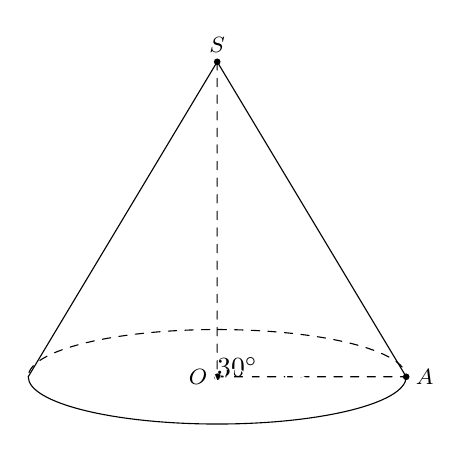
\begin{tikzpicture}[>=stealth,line join=round,line cap=round,font=\footnotesize,scale=0.8,smooth]
			\def\x{3} % Bán kính trụ lớn
			\pgfmathsetmacro{\y}{\x/4} % Bán kính trục bé
			\def\h{5} % Chiều cao
			\coordinate[label=left:$O$] (O) at (0,0);
			\coordinate[label=right:$A$] (A) at (\x,0);
			\coordinate[label=above:$S$] (S) at (0,\h);
			\draw (A) arc (0:-180:{\x} and {\y})--(S)--cycle;
			\draw[dashed] (S)--(O)--(A) arc (0:180:{\x} and {\y});
			\foreach \diem in {A,S,O}	\fill (\diem)circle(1.5pt);
			\tkzMarkAngles[size=1.2cm,opacity=.7,draw=black,mksize=2](O,S,A) 
			\tkzLabelAngle[pos=1](O,S,A){$30^\circ$} 										
			\begin{scope} \path[white]node{MDD-108};\end{scope}
\end{tikzpicture}
		}
	}
\end{ex}

\begin{ex}%[Thi thử lần 2, Sở GD và ĐT - Vĩnh Phúc, PTTH Tam dương, 2020-2021]%[nguyễn hoàng thanh, 12EX3]%[2D2B5-1]
	Phương trình $ \log_3 (3x-2)=3 $ có nghiệm là
	\choice
	{$x=\dfrac{25}{3}$}
	{$x=87$}
	{\True$x=\dfrac{29}{3}$}
	{ $x=\dfrac{11}{3}$}
	\loigiai{
		Điều kiện $ 3x-2>0\Leftrightarrow x>\dfrac{2}{3} $.\\
		Phương trình đã cho tương đương với $ 3x-2=3^3=27\Leftrightarrow x=\dfrac{29}{3}$.
	}
\end{ex}

\begin{ex}%[Thi thử lần 2, Sở GD và ĐT - Vĩnh Phúc, PTTH Tam dương, 2020-2021]%[nguyễn hoàng thanh, 12EX3]%[2D2B5-2]
	Biết $ 4^x+4^{-x}=23$. Tính giá trị của biểu thức $ P=2^x+2^{-x} $.
	\choice
	{$25$}
	{$\sqrt{27}$}
	{$\sqrt{23}$}
	{\True$5$}
	\loigiai{
		Ta có $ 4^x+4^{-x}=23\Leftrightarrow 4^x+2\cdot 2^x\cdot 2^{-x}+ 4^{-x} =25\Leftrightarrow \left( 2^x+2^{-x}\right)^2=25\Leftrightarrow 2^x+2^{-x}=5 $.
	}
\end{ex}

\begin{ex}%[Thi thử L2, Chuyển đề THPT Tam Dương - Vĩnh Phúc, 2021]%[Quan Văn Ón,12EX-3-2021]%[2H1B3-2]
	Cho hình chóp $S.ABCD$ có đáy $ABCD$ là hình thang vuông tại $A$ và $D$. Cạnh bên $SA$ vuông góc với mặt phẳng đáy, $AD = DC = a$, $AB = 2a$, cạnh $SC$ hợp với đáy một góc $30^\circ$. Tính thể tích khối chóp $S.ABC$ theo $a$?
	\choice
	{$\dfrac{a^3}{3}$}
	{$\dfrac{a^3\sqrt{6}}{6}$}
	{$\dfrac{a^3\sqrt{6}}{3}$}
	{\True $\dfrac{a^3\sqrt{6}}{9}$}
	\loigiai{
		\immini{
			Xét $\triangle ACD$ vuông tại $D$ có\\
			$AC = \sqrt{AD^2 + AC^2} = \sqrt{a^2 + a^2} = a\sqrt{2}$.\\
			Vì $SA \perp (ABCD)$ nên $SA \perp AC$\\
			$\Rightarrow \triangle SAC$ vuông tại $A$.\\
			Xét $\triangle SAC$ vuông tại $A$ có \\
			$SA = AC \cdot \tan 30^\circ = a\sqrt{2}\cdot \dfrac{\sqrt{3}}{3} = \dfrac{a\sqrt{6}}{3}$.\\
			Từ $C$, kẻ $CM \parallel AD$ mà $AD \perp AB$ nên $CM \perp AB$, từ đó $AMCD$ là hình chữ nhật. Hơn nữa, hình chữ nhật $AMCD$ có $AD = DC = a$, nên $AMCD$ là hình vuông. Suy ra, $CM = a$.
		}{
			\begin{tikzpicture}[>=stealth, line join=round, line cap = round,scale = 0.8]
			\tkzDefPoints{0/0/A, 7/0/B, -1.5/-2/D, 0/4/S,2/-2/C}
			\tkzDefMidPoint(A,B)\tkzGetPoint{M}
			\tkzDrawSegments(B,C C,D S,B S,C S,D)
			\tkzDrawSegments[dashed](A,B S,A A,C A,D C,M)
			\tkzLabelPoints[left](A)
			\tkzLabelPoints[below](C,D)
			\tkzLabelPoints[right](B)
			\tkzLabelPoints[above](S,M)
			\tkzDrawPoints(S,A,B,C,D,M)
			\tkzMarkRightAngles(S,A,B S,A,D C,D,A D,A,B)
			\tkzMarkAngles[size=0.8cm](S,C,A)
			\node at ($(C)+(120:1.2)$)[scale=0.7]{$30^{\circ}$};
			\tkzMarkSegments[mark=|](M,A M,B)
			\tkzLabelSegment[left](D,A){$a$}
			\tkzLabelSegment[below](D,C){$a$}
			\begin{scope} \path[white]node{MDD-108};\end{scope}
\end{tikzpicture}
		}
		\noindent
		Ta có $S_{\triangle ABC} = \dfrac{1}{2} CM \cdot AB = \dfrac{1}{2} \cdot a \cdot 2a = a^2$.\\
		$\Rightarrow V_{S.ABC} = \dfrac{1}{3}SA \cdot S_{\triangle ABC} = \dfrac{1}{3}\cdot \dfrac{a\sqrt{6}}{3}\cdot a^2 = \dfrac{a^3\sqrt{6}}{9}$ (đvtt).
	}
\end{ex}

\begin{ex}%[Thi thử L2, Chuyển đề THPT Tam Dương - Vĩnh Phúc, 2021]%[Quan Văn Ón,12EX-3-2021]%[2D1B3-6]
	Một vật chuyển động theo quy luật $S = -t^3 + 9t^2 + t + 10$, với $t$ (giây) là khoảng thời gian tính từ lúc vật bắt đầu chuyển động và $S$ (mét) là quãng đường vật đi được trong khoảng thời gian đó. Hỏi trong khoảng thời gian $12$ giây, kể từ lúc bắt đầu chuyển động tại thời điểm $t$ bằng bao nhiêu giây thì vật đạt vận tốc lớn nhất?
	\choice
	{\True $t = 3$s}
	{$t = 6$s}
	{$t = 5$s}
	{$t = 2$s}
	\loigiai{
		\textbf{Nhắc lại:} Đạo hàm cấp một của quãng đường là vận tốc.\\
		Theo đề bài, cần tìm $t$ để vận tốc lớn nhất trong khoảng thời gian $12$ giây, nghĩa là, cần tìm $t\in [0;12]$ để vận tốc lớn nhất.\\
		Xét $v(t) = S' = -3t^2 + 18t + 1$. Khi đó
		$v'(t) = -6t + 18$.\\
		$v'(t) = 0 \Leftrightarrow -6t + 18 = 0 \Leftrightarrow t = 3$.\\
		Ta có $v(0) = 1$; $v(3) = 28$; $v(12) = -215$.\\
		Bảng biến thiên
		\begin{center}
			
\begin{tikzpicture}[scale=0.85, font=\footnotesize, line join=round, line cap=round, >=stealth]
			\tkzTabInit[nocadre=false,lgt=1.2,espcl=2.5,deltacl=0.6]
			{$t$/0.6,$v'(t)$/0.6,$v(t)$/2}
			{$0$,$3$,$12$}
			\tkzTabLine{ ,+,0,-, }
			\tkzTabVar{-/$1$,+/$28$,-/$-215$}
			\begin{scope} \path[white]node{MDD-108};\end{scope}
\end{tikzpicture}
		\end{center}
		$\Rightarrow \max\limits_{t\in\mathscr [0;12]} v(t) = v(3)$.\\
		Như vậy, trong khoảng thời gian $12$ giây, kể từ lúc bắt đầu chuyển động tại thời điểm $t = 3$ giây thì vật đạt vận tốc lớn nhất.
	}
\end{ex}

\begin{ex}%[Thi thử L2, Chuyển đề THPT Tam Dương - Vĩnh Phúc, 2021]%[Quan Văn Ón,12EX-3-2021]%[2D1B2-2]
	Cho hàm số $y = f(x)$ có bảng biến thiên như hình dưới
	\begin{center}
		
\begin{tikzpicture}[scale=0.85, font=\footnotesize, line join=round, line cap=round, >=stealth]
		\tkzTabInit[nocadre=false,lgt=1.2,espcl=2.5,deltacl=0.6]
		{$x$/0.6,$y'$/0.6,$y$/2}
		{$-\infty$,$-1$,$3$,$+\infty$}
		\tkzTabLine{ ,+,0,-,0,+, }
		\tkzTabVar{-/$-\infty$,+/$5$,-/$1$,+/$+\infty$}
		\begin{scope} \path[white]node{MDD-108};\end{scope}
\end{tikzpicture}
	\end{center}
	Số điểm cực trị của hàm số $y = f(x^2 - 4x + 1)$
	\choice
	{$1$}
	{\True $5$}
	{$3$}
	{$2$}
	\loigiai{
		Đặt	$g(x) = f(x^2 - 4x + 1)$.\\
		Ta có $g'(x) = (2x - 4)f'(x^2 - 4x + 1)$.\\
		$\Rightarrow g'(x) = 0 \Leftrightarrow \hoac{&2x - 4 = 0\\&f'(x^2 - 4x + 1) = 0} \Leftrightarrow \hoac{&x = 2\\&x^2 - 4x + 1 = -1\\&x^2 - 4x + 1 = 3} \Leftrightarrow \hoac{&x = 2\\&x =2 - \sqrt{2}\\&x = 2 + \sqrt{2}\\&x = 2 - \sqrt{6}\\&x = 2 + \sqrt{6}.}$\\
		Bảng biến thiên
		\begin{center}
			
\begin{tikzpicture}[scale=0.85, font=\footnotesize, line join=round, line cap=round, >=stealth]
			\tkzTabInit[nocadre=false,lgt=1.2,espcl=2.5,deltacl=0.6]
			{$x$/0.6,$g'(x)$/0.6,$g(x)$/2}
			{$-\infty$,$2-\sqrt{6}$, $2 - \sqrt{2}$, $2$,$2 + \sqrt{2}$, $2 + \sqrt{6}$,$+\infty$}
			\tkzTabLine{ ,-,0,+,0,-,0,+,0,-,0,+, }
			\tkzTabVar{+/$+\infty$,-/,+/,-/,+/,-/,+/$+\infty$}
			\begin{scope} \path[white]node{MDD-108};\end{scope}
\end{tikzpicture}
		\end{center}
		Dựa vào bảng biến thiên, ta thấy, hàm số có $5$ cực trị.
	}
\end{ex}

\begin{ex}%[Thi thử L2, Chuyển đề THPT Tam Dương - Vĩnh Phúc, 2021]%[Quan Văn Ón,12EX-3-2021]%[2D1B1-3]
	Cho hàm số $y = -x^3 - mx^2 + (4m + 9)x + 5$, với $m$ là tham số. Có bao nhiêu giá trị nguyên của $m$ để hàm số nghịch biến trên $\mathbb{R}$?
	\choice
	{$6$}
	{$4$}
	{\True $7$}
	{$5$}
	\loigiai{
		Ta có $y' = -3x^2 - 2mx + 4m + 9$.\\
		Xét $f(x) = y' = -3x^2 - 2mx + 4m + 9$.\\
		Để hàm số nghịch biến trên $\mathbb{R}$ thì $y' \leq 0$, $\forall x \in \mathbb{R}$ $\Leftrightarrow f(x) \leq 0$,  $\forall x \in \mathbb{R}$.\\
		Ta có
		$$f(x) \leq 0,  \forall x \in \mathbb{R} \Leftrightarrow \heva{&a <0 \\&\Delta \leq 0} \Leftrightarrow \heva{&-3 < 0 \quad \textrm{(luôn đúng)}\\&m^2 + 12m + 27 \leq 0} \Leftrightarrow -9 \leq m \leq -3.$$
		$\Rightarrow m \in \left\lbrace -9; -8; -7; -6; -5; -4; -3 \right\rbrace $.\\
		Vậy có $7$ giá trị nguyên của $m$ để hàm số đã cho nghịch biến trên $\mathbb{R}$.
	}
\end{ex}

\begin{ex}%[Thi thử L2, Chuyển đề THPT Tam Dương - Vĩnh Phúc, 2021]%[Quan Văn Ón,12EX-3-2021]%[2D1B5-3]
	Cho hàm số $y = f(x)$ có đồ thị là đường cong như hình vẽ bên. Tìm tất cả các giá trị thực của $m$ để phương trình $2|f(x)| - 2m = 0$ có $4$ nghiệm phân biệt.
	\begin{center}
		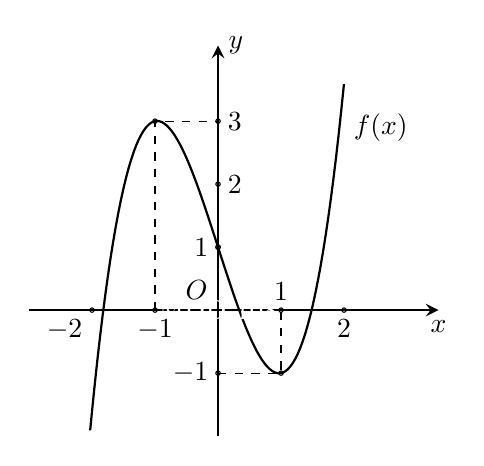
\begin{tikzpicture}[scale = 0.8,>=stealth]
		\draw[->,line width = 1pt] (-3,0)--(0,0) node[above left]{$O$}--(3.5,0) node[below]{$x$};
		\draw[->,line width = 1pt] (0,-2)--(0,4.2) node[right]{$y$};
		\foreach \x in {2,3}{
			\draw (0,\x) node[right]{$\x$} circle (1pt);
		}
		\foreach \x in {-1,1}{
			\draw (0,\x) node[left]{$\x$} circle (1pt);
		}
		\foreach \x in {-1,2}{
			\draw (\x,0) node[below]{$\x$} circle (1pt);
		}
		\draw (-2,0) node[below left]{$-2$} circle (1pt);
		\draw (1,0) node[above]{$1$} circle (1pt);
		\draw (-1,3) circle (1pt);
		\draw (1,-1) circle (1pt);
		\draw (0,1) circle (1pt);
		\draw [thick, domain=-2.03:2, samples=100] %
		plot (\x, {1.1*(\x)^3 - 3.1*(\x)+1});
		\draw [dashed] (-1,0)--(-1,3)--(0,3);
		\draw[dashed] (0,-1)--(1,-1)--(1,0);
		\draw (2,2.9) node[right]{$f(x)$};
		\begin{scope} \path[white]node{MDD-108};\end{scope}
\end{tikzpicture}
	\end{center}
	\choice
	{\True $1 < m < 3$}
	{Không có giá trị nào của $m$}
	{$0 < m < 3$}
	{$1 < m \leq 3$}
	\loigiai{
		\immini{Ta có $2|f(x)| - 2m = 0 \Leftrightarrow |f(x)| = m$.\\
			Dựa vào đồ thị bên dưới, ta thấy, để phương trình $|f(x)| = m$ có $4$ nghiệm phân biệt thì $1 < m < 3$.
		}{
			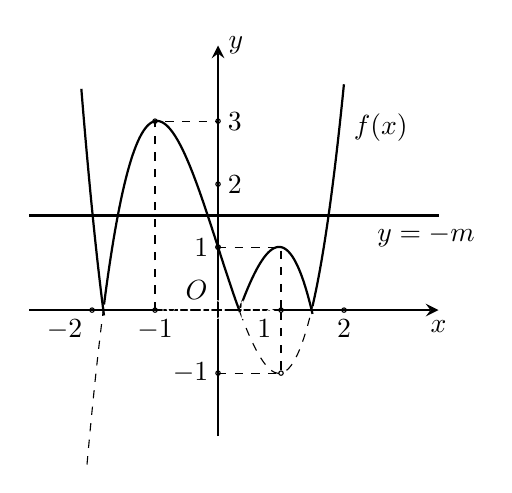
\begin{tikzpicture}[scale = 0.8,>=stealth]
			\draw[->,line width = 1pt] (-3,0)--(0,0) node[above left]{$O$}--(3.5,0) node[below]{$x$};
			\draw[->,line width = 1pt] (0,-2)--(0,4.2) node[right]{$y$};
			\foreach \x in {2,3}{
				\draw (0,\x) node[right]{$\x$} circle (1pt);
			}
			\foreach \x in {-1,1}{
				\draw (0,\x) node[left]{$\x$} circle (1pt);
			}
			\foreach \x in {-1,2}{
				\draw (\x,0) node[below]{$\x$} circle (1pt);
			}
			\draw (-2,0) node[below left]{$-2$} circle (1pt);
			\draw (1,0) node[below left]{$1$} circle (1pt);
			\draw (-1,3) circle (1pt);
			\draw (1,-1) circle (1pt);
			\draw (0,1) circle (1pt);
			\draw [thick, domain=-2.17:-1.81, samples=100] %
			plot (\x, {-1.1*(\x)^3 + 3.1*(\x)-1});
			\draw [dashed, domain=-2.08:-1.81, samples=100] %
			plot (\x, {1.1*(\x)^3 - 3.1*(\x)+1});
			\draw [thick, domain=-1.81:0.35, samples=100] %
			plot (\x, {1.1*(\x)^3 - 3.1*(\x)+1});
			\draw [thick, domain=0.35:1.5, samples=100] %
			plot (\x, {-1.1*(\x)^3 + 3.1*(\x)-1});
			\draw [dashed, domain=0.35:1.5, samples=100] %
			plot (\x, {1.1*(\x)^3 - 3.1*(\x)+1});
			\draw [thick, domain=1.5:2, samples=100] %
			plot (\x, {1.1*(\x)^3 - 3.1*(\x)+1});
			\draw [dashed] (-1,0)--(-1,3)--(0,3);
			\draw[dashed] (0,-1)--(1,-1)--(1,0);
			\draw[dashed] (0,1)--(1,1)--(1,0);
			\draw (2,2.9) node[right]{$f(x)$};
			\draw[-,line width = 1pt] (-3,1.5)--(3.5,1.5);
			\draw (3.3,1.5) node[below]{$y = -m$};
			\begin{scope} \path[white]node{MDD-108};\end{scope}
\end{tikzpicture}
		}
	}
\end{ex}

\begin{ex}%[Thi thử L2, Chuyển đề THPT Tam Dương - Vĩnh Phúc, 2021]%[Quan Văn Ón,12EX-3-2021]%[2D1B5-5]
	Cho hàm số $y = f(x)$ có đồ thị của hàm số $f'(x)$ như sau
	\begin{center}
		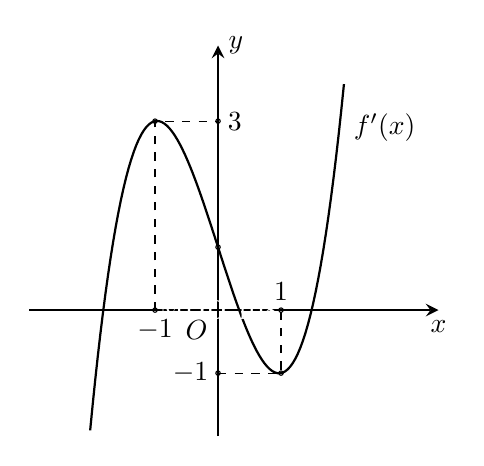
\begin{tikzpicture}[scale = 0.8,>=stealth]
		\draw[->,line width = 1pt] (-3,0)--(0,0) node[below left]{$O$}--(3.5,0) node[below]{$x$};
		\draw[->,line width = 1pt] (0,-2)--(0,4.2) node[right]{$y$};
		\foreach \x in {3}{
			\draw (0,\x) node[right]{$\x$} circle (1pt);
		}
		\foreach \x in {-1}{
			\draw (0,\x) node[left]{$\x$} circle (1pt);
		}
		\foreach \x in {-1}{
			\draw (\x,0) node[below]{$\x$} circle (1pt);
		}
		\draw (1,0) node[above]{$1$} circle (1pt);
		\draw (-1,3) circle (1pt);
		\draw (1,-1) circle (1pt);
		\draw (0,1) circle (1pt);
		\draw [thick, domain=-2.03:2, samples=100] %
		plot (\x, {1.1*(\x)^3 - 3.1*(\x)+1});
		\draw [dashed] (-1,0)--(-1,3)--(0,3);
		\draw[dashed] (0,-1)--(1,-1)--(1,0);
		\draw (2,2.9) node[right]{$f'(x)$};
		\begin{scope} \path[white]node{MDD-108};\end{scope}
\end{tikzpicture}
	\end{center}
	Trên khoảng $(-10;10)$ có tất cả bao nhiêu số nguyên của $m$ để hàm số $g(x) = f(x) + mx + 2020$ có đúng một cực trị?
	\choice
	{\True $16$}
	{$15$}
	{$14$}
	{$13$}
	\loigiai{
		$g(x) = f(x) + mx + 2020$.\\
		$g'(x) = f'(x) + m$.\\
		$\Rightarrow g'(x) = 0 \Leftrightarrow f'(x) = -m$.\\
		Dựa vào đồ thị, để hàm số $g(x)$ có đúng một cực trị thì $\hoac{&-m \geq 3\\&-m \leq -1} \Leftrightarrow \hoac{&m \leq -3\\&m \geq 1.}$\\
		mà $m \in (-10;10)$ nên $m \in \left\lbrace -9;-8;-7;-6;-4;-3;1;2;3;4;5;6;7;8;9 \right\rbrace $.\\
		Vậy có tất cả $16$ số nguyên của $m$ để hàm số $g(x) = f(x) + mx + 2020$ có đúng một cực trị.
	}
\end{ex}

\begin{ex}%[Đề thi HK1, Trường THPT Tam Dương, Vĩnh Phúc năm 2020-2021]%[Dự án 12EX3-Nguyễn Anh Quốc]%[2D2K4-1]
	Tìm tất cả các giá trị thực của tham số $m$ để hàm số $y=\log\left(x^2-2mx+4\right)$ có tập xác định là $\mathbb{R}$.
	\choice
	{$-2\le m\le 2$}
	{$m=2$}
	{$m>2$ hoặc $m<-2$}
	{\True $-2<m<2$}
	\loigiai{
		Hàm số có tập xác định là $\mathbb{R}$ khi và chỉ khi 
		{\allowdisplaybreaks
			\begin{align*}
				x^2-2mx+4>0,\forall x\in \mathbb{R}\Leftrightarrow \heva{&a=1>0\\&\Delta'=m^2-4<0}\Leftrightarrow -2<m<2.
		\end{align*}}	
	}
\end{ex}

\begin{ex}%[Thi thử lần 2, Sở GD và ĐT - Vĩnh Phúc, PTTH Tam dương, 2020-2021]%[nguyễn hoàng thanh, 12EX3]%[2D1K4-1]
	Số tiệm cận đứng của đồ thị hàm số $ y=\dfrac{\sqrt{x+9}-3}{x^2+x} $ là
	\choice
	{$ 3 $}
	{$ 2 $}
	{$ 0 $}
	{\True $ 1 $}
	\loigiai{
		Ta có $ x^2+x=0\Leftrightarrow x=0; x=-1 $.\\
		Giới hạn
		\begin{itemize}
			\item $ \lim\limits_{x\to 0}\dfrac{\sqrt{x+9}-3}{x^2+x}=\lim\limits_{x\to 0}\dfrac{x}{x(x+1)(\sqrt{x+9}+3)}=\lim\limits_{x\to 0}\dfrac{1}{(x+1)(\sqrt{x+9}+3)}=\dfrac{1}{6}$, suy ra $ x=0 $ không phải là tiệm cận đứng.
			\item $ \lim\limits_{x\to-1^+}\dfrac{\sqrt{x+9}-3}{x^2+x}=-\infty$; $ \lim\limits_{x\to-1^-}\dfrac{\sqrt{x+9}-3}{x^2+x}=+\infty$, suy ra $ x=-1 $ là tiệm cận đứng.
		\end{itemize}
	}
\end{ex}

\begin{ex}%[Thi thử lần 2, Sở GD và ĐT - Vĩnh Phúc, PTTH Tam dương, 2020-2021]%[nguyễn hoàng thanh, 12EX3]%[2D1K2-2]
	\immini{Cho hàm số $ y=f(x) $. Hàm số $ y=f'(x) $ có đồ thị như hình bên. Hàm số $ y=f(x) $ có bao nhiêu điểm cực trị?}{
		\begin{tikzpicture}[>=stealth,line join=round,line cap=round,font=\footnotesize,scale=0.7,smooth]
		\draw[->] (-3,0)--(5,0)node[below]{$x$};
		\foreach \x in {-2,-1,1,2,3,4}\draw[shift={(\x,0)}] (0,2pt)--(0,-2pt) node[below]{\scriptsize $\x$};
		\draw[->] (0,-2.5)--(0,3.5)node[right]{$y$};
		\draw[] plot[smooth,tension=.65] coordinates{(-1.7,-2) (-1,0) (0,.7) (1,0)(2.7,-1.2)(4,0) (5,2.5)}node[right]{$y=f'(x)$};
		\begin{scope} \path[white]node{MDD-108};\end{scope}
\end{tikzpicture}
	}
	\choice
	{$2$}
	{\True$3$}
	{$0$}
	{ $1$}
	\loigiai{
		\immini{Dựa vào đồ thị, ta có bảng biến thiên như hình vẽ. \\
			Căn cứ vào bảng biến thiên ta thấy hàm số có $ 3 $ điểm cực trị.}{% Cần khai báo \usepackage{tkz-tab}
			
\begin{tikzpicture}[scale=.8, font=\footnotesize, line join=round, line cap=round, >=stealth]
			\tkzTabInit[nocadre=false,lgt=1,espcl=2,deltacl=0.5]{$x$/.7 ,$y'$/.7,$y$/2}
			{$-\infty$ , $-1$ , $1$, $ 4 $, $+\infty$}
			\tkzTabLine{ , - , $0$ ,+, $ 0 $, -, $0$ , + , }
			\tkzTabVar{+/$+\infty$ , -/$f(-1)$ ,+/$f(-1)$ ,-/$ f(4) $, +/$+\infty$}
			\begin{scope} \path[white]node{MDD-108};\end{scope}
\end{tikzpicture}}
		
	}
\end{ex}

\begin{ex}%[Thi thử lần 2, Sở GD và ĐT - Vĩnh Phúc, PTTH Tam dương, 2020-2021]%[nguyễn hoàng thanh, 12EX3]%[2D1K4-1]
	\immini{Cho hàm số $ y=f(x) $ có đồ thị như hình vẽ. Đồ thị hàm số $ g(x)=\dfrac{2020}{2f(x)+1} $ có số đường tiệm cận đứng là}{
		\begin{tikzpicture}[scale=.8, font=\footnotesize, line join=round, line cap=round, >=stealth]
		\def\a{1} 
		\def\b{2}
		\def\c{1}
		\draw[->] (-3,0) -- (3,0) node[below] {\scriptsize $x$};
		\draw[->] (0,-3) -- (0,2) node[left] {\scriptsize $y$};
		\draw 
		(0,0)node[below right]{\scriptsize$O$}
		(-1,0)node[above]{\scriptsize$-1$} (1,0)node[above]{\scriptsize$1$}
		(0,-1)node[below right]{\scriptsize$-1$};
		\clip (-3,-3)rectangle(3,3);
		\draw[samples=200,smooth,domain=-4:4] plot(\x,{-\a*(\x)^4+(\b)*(\x)^2 -\c});
		\begin{scope} \path[white]node{MDD-108};\end{scope}
\end{tikzpicture}
	}
	\choice
	{$2$}
	{$3$}
	{\True$4$}
	{$5$}
	\loigiai{
		Cho $ 2f(x)+1=0\Leftrightarrow f(x)=-\dfrac{1}{2} $.\\
		Dựa vào đồ thị hàm số, ta thấy đường thẳng $ y=-\dfrac{1}{2} $ cắt đồ thị hàm số tại $ 4 $ điểm, suy ra phương trình $ 2f(x)+1=0 $ có bốn nghiệm, suy ra $ g(x) $ có $ 4 $ tiệm cận đứng. 
	}
\end{ex}

\begin{ex}%[Thi thử lần 2, Sở GD và ĐT - Vĩnh Phúc, PTTH Tam dương, 2020-2021]%[nguyễn hoàng thanh, 12EX3]%[2D2K5-2]
	Cho phương trình $ \log_9 x^2-\log_3(5x-1)=-\log_3m $. Có tất cả bao nhiêu giá trị nguyên của $ m $ để phương trình đã cho có nghiệm?
	\choice
	{\True$4$}
	{$6$}
	{Vô số}
	{$5$}
	\loigiai{
		Điều kiện $ x>\dfrac{1}{5} $ và $ m>0 $.\\
		Với điều kiện trên phương trình đã cho tương đương với $$ \log_3 x-\log_3 (5x-1)=-\log_3 m\Leftrightarrow \dfrac{x}{5x-1}=\dfrac{1}{m}
		\Leftrightarrow m=5-\dfrac{1}{x}.$$
		Vì $ m\in \mathbb{Z} $ suy ra $\heva{& \dfrac{1}{x}\in\mathbb{N}\\& x>\dfrac{1}{5} }$ suy ra $ 1\le \dfrac{1}{x}<5\Leftrightarrow \dfrac{1}{x}\in \left\lbrace 1;2;3;4\right\rbrace $.\\
		Với 
		\begin{itemize}
			\item $ \dfrac{1}{x}=1\Rightarrow m=4 $.
			\item $ \dfrac{1}{x}=2\Rightarrow m=3 $.
			\item $ \dfrac{1}{x}=3\Rightarrow m=2 $.
			\item $ \dfrac{1}{x}=4\Rightarrow m=1 $.
		\end{itemize}
	}
\end{ex}

\begin{ex}%[Thi thử L2, Chuyển đề THPT Tam Dương - Vĩnh Phúc, 2021]%[Quan Văn Ón,12EX-3-2021]%[2H2K1-1]
	Một hình trụ có thiết diện qua trục là hình vuông, diện tích xung quanh bằng $36\pi a^2$. Tính thể tích $V$ của lăng trụ lục giác đều nội tiếp hình trụ.
	\choice
	{$27\sqrt{3}a^3$}
	{$24\sqrt{3}a^3$}
	{$36\sqrt{3}a^3$}
	{\True $81\sqrt{3}a^3$}
	\loigiai{
		\immini{
			Giả sử hình ta đang xét là hình bên.\\
			Vì hình trụ có thiết diện qua trục là hình vuông, do đó, đường kính và đường cao bằng nhau, nghĩa là $2r = h \Rightarrow S_{\textrm{xq}} = 2\pi r h = \pi h^2$.\\
			$\Rightarrow S_{\textrm{xq}} = 36\pi a^2 \Leftrightarrow \pi h^2 = 36\pi a^2 \Leftrightarrow h = 6a \Rightarrow r = 3a$.\\
			Vì lăng trụ lục giác đều nội tiếp hình trụ nên lục giác nội tiếp đường tròn đáy, do đó, mỗi tam giác tạo bởi hai bán kính liên tiếp là tam giác cân với đỉnh là tâm đường tròn đáy và mỗi góc tạo bởi 2 bán kính liên tiếp là $360^\circ : 6 = 60^\circ$, suy ra, mỗi tam giác là tam giác đều và các tam giác này bằng nhau.\\
			$\Rightarrow S_{\textrm{lục giác}} = 6\cdot S_{O'C'D'} = 6\cdot \dfrac{\sqrt{3}}{4}\cdot (3a)^2 = \dfrac{27a^2\sqrt{3}}{2}$.\\
			$\Rightarrow V_{\textrm{lăng trụ}} = S_{\textrm{lục giác}}\cdot h = \dfrac{27a^2\sqrt{3}}{2} \cdot 6a = 81a^3\sqrt{3}$.
		}{
			\begin{tikzpicture}[scale=0.4, font=\footnotesize, line join=round, line cap=round, >=stealth]
			\def\x{5} %bán trục lớn
			\def\y{1.3} %bán trục bé
			\def\h{9} %chiều cao trụ
			% ve tam và 2 đỉnh
			\tkzDefPoints{0/0/O,-\x/0/A1,\x/0/B1,0/\h/O'}
			% vẽ elip
			\draw[dashed] (B1) arc (0:180:\x cm and \y cm);
			\draw (B1) arc (0:-180:\x cm and \y cm);
			% tịnh tiến lên trên 
			\tkzDefPointBy[translation=from O to O'](A1) \tkzGetPoint{A1'}
			\tkzDefPointBy[translation=from O to O'](B1) \tkzGetPoint{B1'}
			% vẽ elip trên
			\draw (B1') arc (0:360:\x cm and \y cm);
			
			%%% dung luc giac day duoi
			\coordinate (A) at ($(O)+({\x*cos(150)},{\y*sin(150)})$);
			\coordinate (B) at ($(O)+({\x*cos(105)},{\y*sin(105)})$);
			\coordinate (C) at ($(O)+({\x*cos(60)},{\y*sin(60)})$);
			\tkzDefPointBy[translation=from A to O](O) \tkzGetPoint{D}
			\tkzDefPointBy[translation=from B to O](O) \tkzGetPoint{E}
			\tkzDefPointBy[translation=from C to O](O) \tkzGetPoint{F}
			%%% dung luc giac day tren
			\tkzDefPointBy[translation=from O to O'](A) \tkzGetPoint{A'}
			\tkzDefPointBy[translation=from O to O'](B) \tkzGetPoint{B'}
			\tkzDefPointBy[translation=from O to O'](C) \tkzGetPoint{C'}
			\tkzDefPointBy[translation=from O to O'](D) \tkzGetPoint{D'}
			\tkzDefPointBy[translation=from O to O'](E) \tkzGetPoint{E'}
			\tkzDefPointBy[translation=from O to O'](F) \tkzGetPoint{F'}
			%%% Danh dau, noi va label cac diem
			\tkzDrawPoints[fill=black](O,O',A,B,C,D,E,F,A',B',C',D',E',F')
			\tkzDrawSegments(A1,A1' B1,B1' A',B' B',C' C',D' D',E' E',F' F',A' F,F' E,E' D,D' A',D' O',C')
			\tkzDrawSegments[dashed](A,B B,C C,D D,E E,F F,A A,A' B,B' C,C' A,D)   
			\tkzLabelPoints[above](O,O', A', B', C')
			\tkzLabelPoints[below](D,E,F)
			\tkzLabelPoints[above right](B,A,C)
			\tkzLabelPoints[below left](D',E',F')
			\draw[dashed] (O) to node[sloped,above]{$r$} (D);
			\draw[dashed] (B1) to node[right]{$h$} (B1');
			\begin{scope} \path[white]node{MDD-108};\end{scope}
\end{tikzpicture}
		}
	}
\end{ex}

\begin{ex}%[Thi thử L2, Chuyển đề THPT Tam Dương - Vĩnh Phúc, 2021]%[Quan Văn Ón,12EX-3-2021]%[2D2K4-2]
	Cho hàm số $f(x) = \ln \dfrac{2018x}{x+1}$. Tính tổng $S = f'(1) + f'(2) + \cdots + f'(2018)$.
	\choice
	{$\ln 2018$}
	{$1$}
	{$2018$}
	{\True $\dfrac{2018}{2019}$}
	\loigiai{
		Ta có $\left( \dfrac{2018x}{x+1} \right)' = \dfrac{2018(x+1) - 2018x}{(x + 1)^2} = \dfrac{2018}{(x+1)^2}$.\\
		$\Rightarrow f'(x) = \left( \ln \dfrac{2018x}{x+1} \right)' = \dfrac{2018}{(x+1)^2} \cdot \dfrac{x+1}{2018x} = \dfrac{1}{x(x+1)} = \dfrac{1}{x} - \dfrac{1}{x+1}$.
		\begin{eqnarray*}
			S = f'(1) + f'(2) + \cdots + f'(2018) &=& \left( \dfrac{1}{1} - \dfrac{1}{2} \right) + \left( \dfrac{1}{2} - \dfrac{1}{3} \right) + \cdots + \left( \dfrac{1}{2018} - \dfrac{1}{2019} \right)\\
			&=& 1 - \dfrac{1}{2019}\\
			&=& \dfrac{2018}{2019}.
		\end{eqnarray*}
	}
\end{ex}
\Closesolutionfile{ans}
\begin{indapan}{10}
	{ans/ans-2-GHK1-23-TamDuong-VinhPhuc-21}
\end{indapan}
